\section{Motivation}

The field of 3D computer graphics has always been a fascinating subject to me. Creating virtual worlds and being able to inspect those from every possible viewpoint is a great way to present almost any object one can think of to a wider audience. I finished my apprenticeship as a A/V media designer, so computer graphics are a helpful tool to e.g. previsualize camera work. The best fact about 3D is that it has so many versatile applications in many fields. 3D information can be retrieved from 2D images, taken with a real photo camera, via photogrammetry and can, in turn, be rendered onto a flat computer screen by rendering a scene with a virtual camera. At the point a object is available as a 3D model, it can be postprocessed in various ways. It can be animated, physically simulated and eventually rendered as a video. With modern display technologies the movie can be played out as a stereoscopic one and viewed with anaglyph (red, cyan), polarized, shutter or even without glasses by using e.g. a parallax barrier display (Wikipedia, \parencite{wiki:ParallaxBarrier}). Furthermore objects can become tangible via 3D printing or can be inspected interactively in games with the help of virtual reality glasses like the Oculus Rift (Oculus VR, \parencite{OculusVR}). It is amazing that anyone can create and enjoy those virtual worlds today.

Additionally, I am highly interested in historical topics. As an active member of a local citizens association and representative of a settlement, where I am always available for any citizenship matters that people might have, I get to know many interesting people and the projects they are working on. Thus I am learning a lot about interesting historical facts and development of culture. Of course, not only about positive history. Especially the history of Langwasser, district of Nuremberg, Germany, is very terrifying and shocking. The district has been formerly used for tent cities and the Märzfeld ("March Field", a representation and parade ground) during the Reich Party Congress in Nuremburg, Germany, between 1933 and 1938 (Wikipedia, \parencite{wiki:NaziPartyRallyGround}). The construction of a railway station, called Bahnhof Märzfeld and placed right in the center of Langwasser, was partly finished in 1938. That station has been used initially to transport the members of the Reich Party Congress to the event. During World War II it was used for the deportation of about 940 people to concentration camps, where only 17 of them survived (Stadtteilforum Langwasser, \parencite{StadtteilforumTafel6}). This railway station is in a ruinous condition at the moment. People go by, without noticing that this is real history, that passes them by. This was a big concern for me, so I started to search for ways to make the history become real again, in an enjoyable way.

And then there was the day I talked to my professor, Mr. Dr. Stefan Röttger, about my wish to use laser scanning for historic 3D reconstruction. Suprisingly my professor told me, that we have a laser scanning device at university which could be used for a thesis. The moment he told me that, was the moment I made my decision to center my thesis around laser scanning.

Lastly, a strong motivational force was discovered after researching how the laser scanner point cloud can be used to create the historic building model based off of a recent laser scan. 3D software enables a user to tweak automatically generated meshes or even to add new geometry. Due to my personal experience with the open source 3D graphics suite Blender and the decreasing interest in other software like Autodesk 3ds Max or Maya in favor of Blender (Google Trends, \parencite{Interest3DSoftware}) it was necessary to work with point clouds in Blender. Unfortunately Blender is not designed to work with point clouds at the time of this writing.

As will be described in greater detail hereafter, the aforementioned facts lead to an initial project specification. 


\section{Initial project specification}

The idea for this research started with the personal concern of reconstructing a historical site like the old railway station in Langwasser in its historic state. Due to the fact that this railway station has never been fully finished and therefore poor historical documentation, a 3D reconstruction wouldn't be complete. Luckily the famous Pellerhaus was the perfect candidate for this research. After its destruction during World War II, it was rebuilt quite differently to the original state. While the inner courtyard is almost finished with reconstruction at the time of this writing, the facade is still looking modern. At that point, it was clear that the main research topic is going to examine ways to reconstruct the Pellerhaus facade in its historic state.
A more concrete specification was defined by considering how this is going to be done. The current state of the building has to be captured with laser scanning technology to get the correct measurements from the real world reference. This point cloud data needs to be processed then. To do so, a custom software is required to be written, which can read a file format exported from the proprietary Faro SCENE application, create a panoramic image representation of the data, use it to generate a 3D mesh and export this mesh to a widely supported file format. This research will mostly rely on the open source software Blender to model and animate the historic state of the Pellerhaus, thus it is crucial to provide a compatible output to be used as a basis for the design process. By creating a textured surface from the point samples, this research will provide a way for the artist to overcome a bad design decision in Blender, which is making it not capable of displaying or rendering colored point clouds at all (see thread by author on BlenderArtists \parencite{webBlenderArtistsPointCloudSupport} ). The goal of this research is to get a 3D model of the Pellerhaus in its historic state from 1605 by utilizing point clouds generated via laser scanning as described before.

\section{Project schedule}

This project is divided into two main phases. The first phase is developing the software for converting laser scanner point clouds as 3D panorama meshes. The second one is designing the historic 3D model from this initial mesh.\\

This is visualized in the following GANTT chart:\\

\definecolor{RoyalBlue}{RGB}{92,102,149}
\definecolor{OliveGreen}{RGB}{51,151,102}
\definecolor{Maroon}{RGB}{180,20,53}
\begin{ganttchart}[
	x unit=1.3cm,
	y unit title=0.7cm,
	y unit chart=0.8cm,
	vgrid, hgrid,
	time slot format=isodate-yearmonth,
	compress calendar,
	title/.append style={draw=none, fill=RoyalBlue!50!black},
	title label font=\sffamily\bfseries\color{white},
	title label node/.append style={below=-1.6ex},
	title left shift=.05,
	title right shift=-.05,
	title height=1,
	bar/.append style={draw=none, fill=OliveGreen!75},
	bar height=.6,
	bar label font=\normalsize\color{black!50},
	group right shift=0,
	group top shift=.6,
	group height=.3,
	group peaks height=.2,
	bar incomplete/.append style={fill=Maroon}
	]{2015-01}{2015-07}
	\gantttitlecalendar{year, month=shortname} \\
	
	\ganttset{progress label text={}, link/.style={black, -to}}
	\ganttbar[progress=100, name=pp]{Laser Scanning}{2015-01-15}{2015-01-25} \\
	
	\ganttgroup{Software development}{2015-02-15}{2015-06-10} \\
	\ganttbar[progress=100, name=T1A]{Import}{2015-02-15}{2015-02-18} \\
	\ganttbar[progress=100]{Processing}{2015-02-19}{2015-03-25} \\
	\ganttbar[progress=100, name=T1C]{Export}{2015-03-24}{2015-04-01} \\
	\ganttbar[progress=100]{Testing / Bugfixing}{2015-02-26}{2015-06-10} \\
	
	\ganttgroup{Video production}{2015-06-08}{2015-07-10} \\
	\ganttbar[progress=100, name=T2A]{Modeling}{2015-06-08}{2015-06-10} \\
	\ganttbar[progress=100]{Animation}{2015-06-10}{2015-07-02} \\
	\ganttbar[progress=100]{Rendering}{2015-06-12}{2015-07-10} \\
	
	\ganttset{link/.style={OliveGreen}}
	\ganttlink[link mid=.4]{pp}{T1A}
	\ganttlink[link mid=.159]{T1C}{T2A}
	\label{tab:project_schedule}
\end{ganttchart}\\


\section{State-of-the-art methods for 3D reconstruction}

There are several methods that allow for the generation of 3D meshes from various data. One can either use several still images or videos, sample the real world with modern sensor technology or use open data for generating geometry of varying complexity. This is described as follows:

\subsection{Light Detection And Ranging (LiDAR)}

The term Light Detection And Ranging (in short LiDAR) is commonly used with high precision applications, such as scanning and mapping of indoor and outdoor environments. It uses a laser beam emitter and receiver. By using the Distance-Speed-Time formula it is very easy to compute how far away an object is:\\

$$  speed = \dfrac{distance}{time} \Longleftrightarrow distance = time * speed $$\\
The time between sending a signal and receiving it is measured and multiplied by the speed of light ($c = 299,792,458 \medspace \frac{m}{s}$, Wikipedia \parencite{wiki:SpeedOfLight}). This returns the meters the light traveled from the emitter to the obstacle and back. Dividing this distance by two yields the range to the obstacle in meters (Schroeder \parencite[see][p8-9]{dp_lidar}).

As this gives the meters to only one specific point, it is necessary to keep measuring from different viewpoints. This can be done by rotating the scanning device horizontally and vertically simultaneously. To keep cables from winding up by using two motors, devices usually use only one motor for the horizontal and a flat mirror on an elliptical mount for the vertical rotation. That way it is possible to sample a lot of points around the device position quickly and effectively.

In this work the LiDAR scanner Faro Focus 3D is being used. It is capable of capturing 976,000 points per second with a vertical and horizontal field of view of 305 and 360 degrees, respectively (Techsheet Faro Focus 3D, \parencite{faro_techsheet}). For allowing a better registration it can also use GPS for localization and a barometer for height measurement. The measured points can be colored with a built-in camera of around 70 Megapixels. The price for the Focus 3D totals at 61,404.37 Euro (Opti-cal Survey Equipment Ltd. \parencite{survey_equipment}).

\begin{figure}[h]
	\centering
	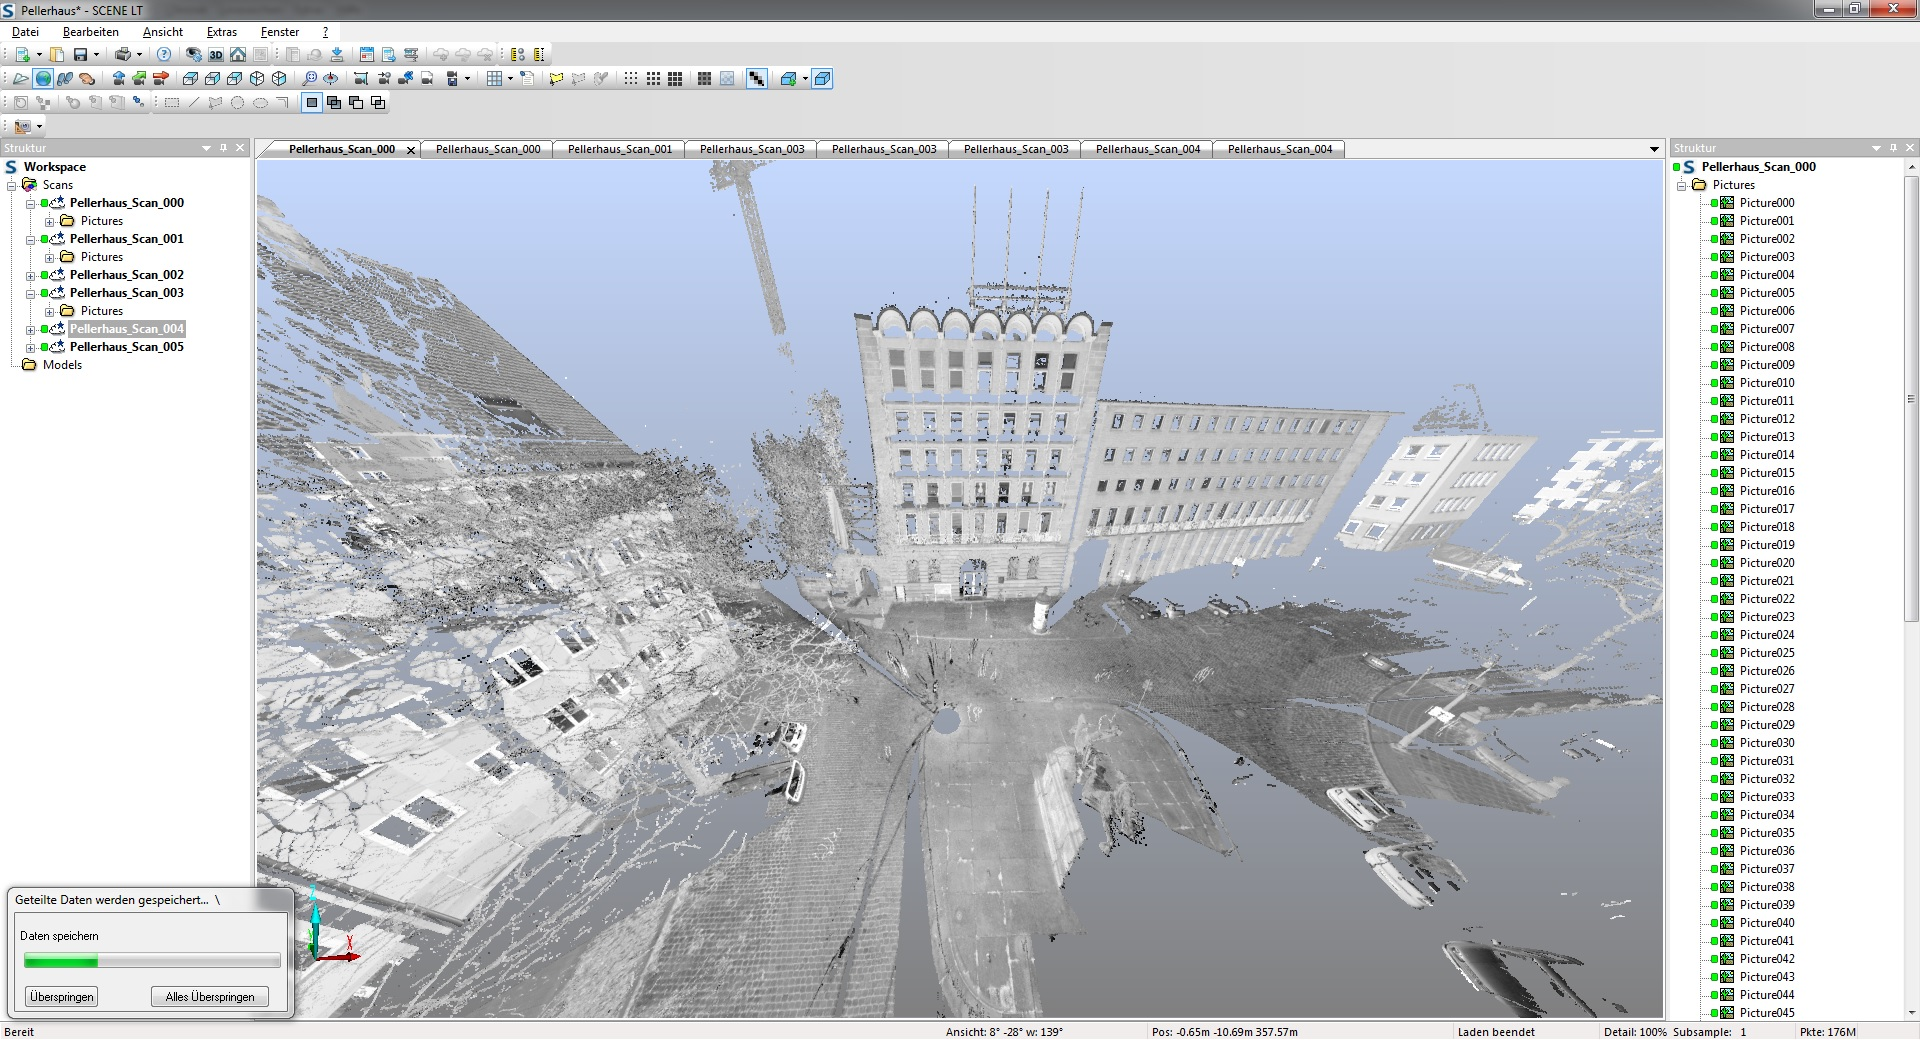
\includegraphics[scale=0.25]{Pellerhaus_FirstGlance.jpg}
	\caption{LiDAR Scanner Point Cloud of the Pellerhaus}
	\label{fig:LiDAR_PointCloud}
\end{figure}

Besides using a stationary device, portable devices are also available. Recently a new technology has been revealed by Csiro and is called \textit{Zebedee}. This handheld laser scanner can be used in challenging environments where a stationary device would require several scans to cover the whole area (e.g. caves, staircases) while the operator is walking. It samples over 40,000 range measurements every second and consists of a 2D laser scanner mounted on a spring system (Mail Online, \parencite{zebedee_info}). Especially the visual effects field has a great use for this device, since the environments can vary a lot during video shootings and a 3D mesh representation is ubiquitous today. The price for the ZEB1 handheld laser scanner is 17,000 Euro\footnote{Source: Personal contact to sales team}.

Although measuring with laser technology can be found in household devices as an alternative for tape measuring, it is still quite complicated to reverse engineer such devices to get the raw distance reading. Fortunately a group of engineers tried to bridge the gap by starting a crowd funding campaign for a low-cost laser range finder, called the LiDAR-Lite (PulsedLight \parencite{pulsedlight}). It has a total range of 40 meters with a resolution of 1 cm. During this research this sensor is being used with a custom arduino build to examine how it can be used as a cheap alternative to the examples mentioned in the beginning. The price for one module is at 82 Euro.

\subsection{Ultrasonic}

In contrast to LiDAR, most ultrasonic sensors are cheap, but generally are not used for higher distances at several tens of meters (though, there are products for a range higher than 100 meter, compare VEGAPULS 69 \parencite{vegapuls}). The reason for this is that sound is usually affected stronger by environmental properties than light (compare Sensors Magazine \parencite{sensorsmag}). Due to this they are often used for shorter distances e.g. for near field obstacle recognition in robotics or in small desktop laser scanners (compare Dinh \parencite{yt_smalldesktoplaser}). Typical ultrasonic sensor modules with a maximum range of around 5 m can be purchased for 5 Euro already.



\subsection{Photogrammetry}

Photogrammetry (also referred to as multi-view reconstruction) is a technique from the Computer Vision field and presents a cost-effective alternative to laser scanning. A real 3D object can be reconstructed as a virtual 3D model by using photographs of the scene and feeding them into such software. This works by detecting image features (for example by using Harris Corner Detector or SIFT algorithms), matching those between image pairs, computing the respective camera positions and re-projecting the reconstructed 3D points to get a point cloud representation of the real photograph (compare Solem \parencite[][p29]{bookProgrammingComputerVisionwithPython}).
The computer vision algorithms get better each day and there is plenty of software using them.

\begin{figure}[h]
	\centering
	\begin{subfigure}[b]{0.3\textwidth}
		\centering
		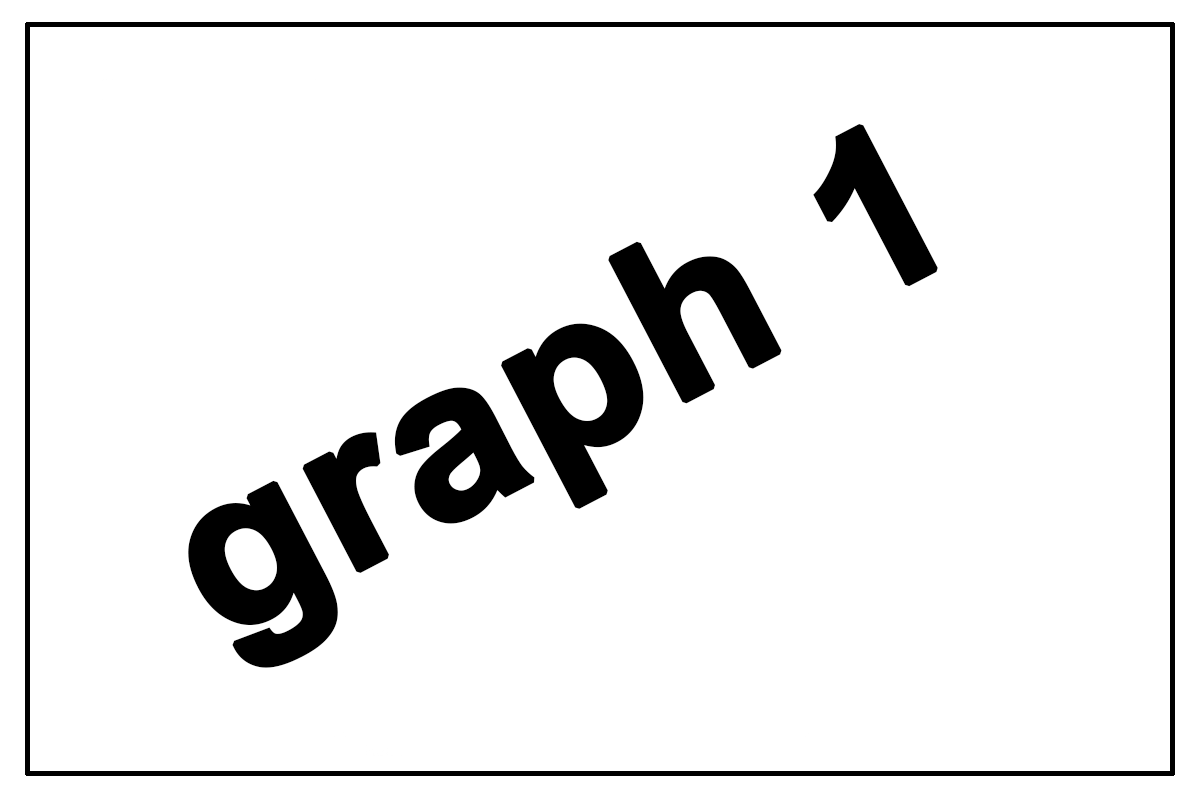
\includegraphics[width=\textwidth]{graph1.png}
		\caption{$OpenSource: Visual SFM + Meshlab$}
		\label{fig:visualsfm meshlab}
	\end{subfigure}
	\hfill
	\begin{subfigure}[b]{0.3\textwidth}
		\centering
		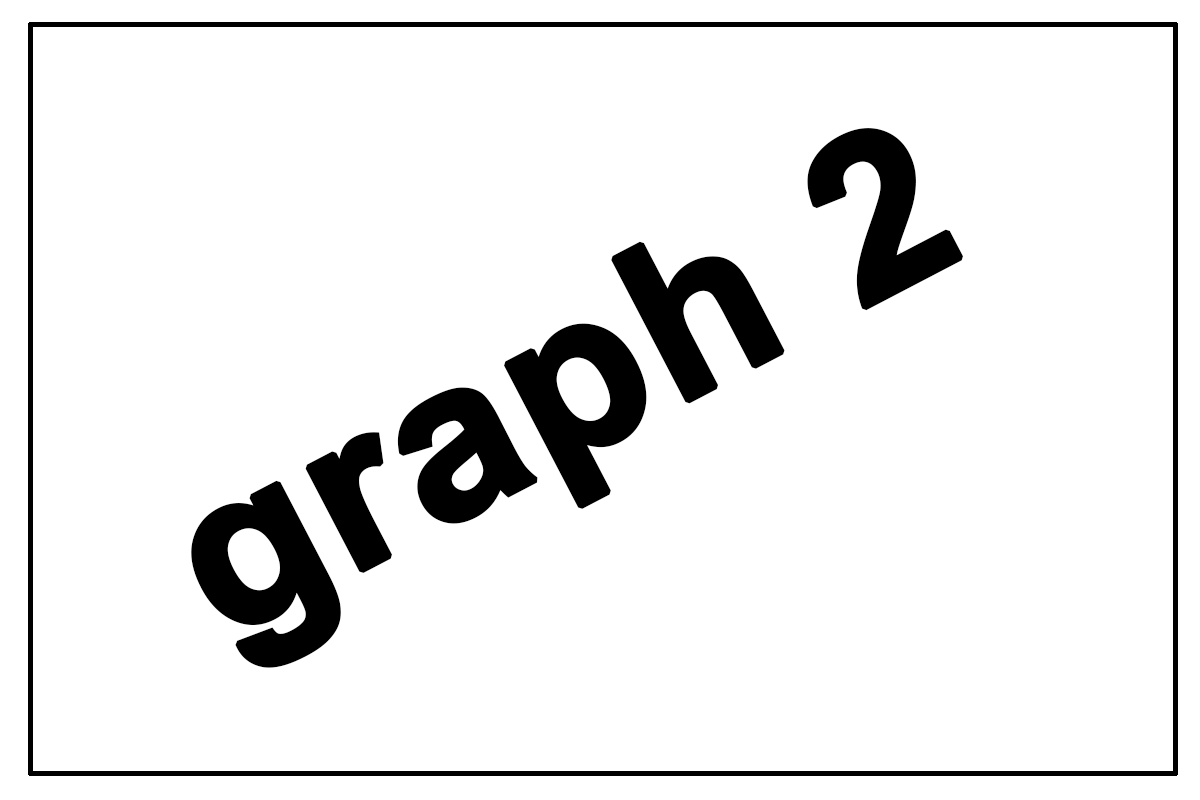
\includegraphics[width=\textwidth]{graph2.png}
		\caption{$Free: Autodesk 123D Catch$}
		\label{fig:123dcatch}
	\end{subfigure}
	\hfill
	\begin{subfigure}[b]{0.3\textwidth}
		\centering
		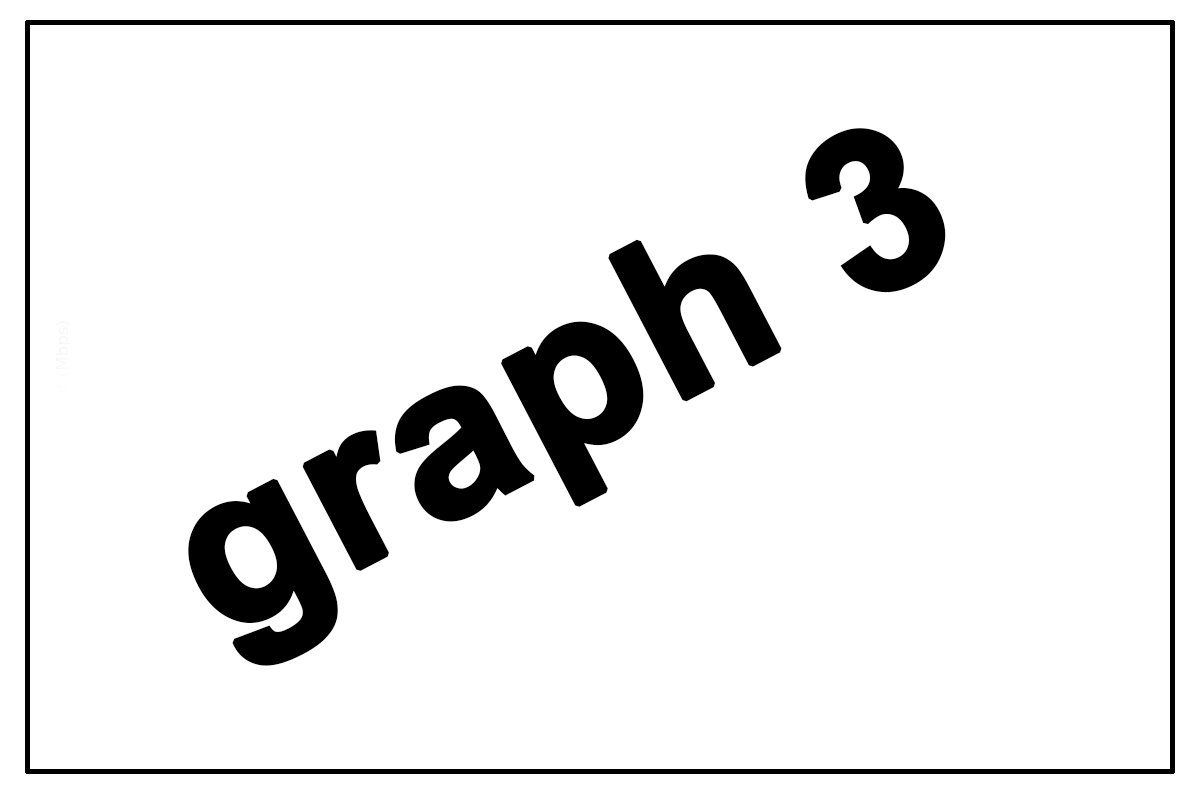
\includegraphics[width=\textwidth]{graph3.png}
		\caption{$Commercial: Agisoft Photoscan Pro (Demo)$}
		\label{fig:photoscan pro}
	\end{subfigure}
	\caption{Multiview Reconstruction from historic stereo pairs}
	\label{fig:multiview reconstruction historic stereo}
\end{figure}

Photogrammetry will be used in this project to try reconstructing surfaces from historical images. Fortunately stereographic image pairs are provided through the Altstadtfreunde Nürnberg e.V. By matching the laser scanner data with the Photogrammetry output a good groundwork is expected to be done for the final surface reconstruction.

\subsection{Google Maps (R) }

The commercial application allows viewing cities from the sky with a rough representation of 3D building shapes (compare Zamora \parencite{google_maps}). While this service had gray boxes some years ago, today the visualization is getting more accurate. It is possible to see small details with better modeled and textured buildings.

\subsection{Open Street Map (R) }

The open source alternative to the commercial service above offers the basic functions for map viewing and navigation. OpenStreetMap (OSM) offers very detailed access to its data, like boundaries, streets and building footprints. That way it is possible to extract simple building shapes (compare F4 \parencite{f4map}) that can be used in custom software free of charge.

To allow for a better mapping of buildings there are also proposals on an indoor version of OSM (compare OpenStreetMap Wiki \parencite{openstreetmap_wiki}). Having this data available is a helpful thing for applications such as indoor navigation at railway and subway stations, mobile emergency exit information and robotics.

\subsection{Bavarian State Office for Survey and Geoinformation}

Geodata and city plans are also provided officially through governmental institutions. They provide various types of data, among others historical aerial photographs, digital elevation models (DEM) and also 3D building shapes. For educational purposes (like i.e. this research) they offer a university discount for the data of 25 percent. A usual dataset without any discounts containing 7580 buildings of Langwasser, district of Nuremberg in Germany, costs 1158 Euro\footnote{Personal research and contact}.

\subsection{Autonomous mapping with UAV's and SLAM}

Drones, or unmanned aerial vehicles (UAV's), are getting more popular each day. Most of them are also equipped with a camera which allows for taking pictures or videos from viewpoints a human cannot reach easily. More expensive drones have LiDAR systems attached (Shen et. al. \parencite{drones_lidar}) which allow - together with the IMU (Inertial Measuring Unit) and GPS (Global Positioning System) to localize it and map its environment. A popular term for this is Simultaneous Localization And Mapping (SLAM).

\subsection{Manual methods}

If all other methods fail, there is still the chance to get a reconstruction done roughly by taking measurements of real objects with measuring tapes or eyeballing. Loading reference pictures from the front, side and top view into a 3D software can already yield decent results.

\section{Defining the scope of this research}

Although this work uses a combination of several techniques (briefly presented above), the main focus is put on examination if panoramic projection of laser scanner point clouds will be an aid for 3D reconstruction or not. This will be evaluated by using the result from the converter in a real world use case of using the generated mesh in the design process.